\section{Interface de Usuário e de Comunicação}
\label{sec:interface}

A comunicação do sistema é realizada via rede Ethernet estruturada com o auxílio de um \textit{switch}, conforme ilustrado na \autoref{fig:arquitetura_hardware}. A padronização do método de transmissão baseia-se no uso de endereçamento IP estático para a placa de medição, o que simplifica a identificação do dispositivo na rede e a integração com a interface. O protocolo adotado para a troca de pacotes é o UDP (\textit{User Datagram Protocol}), escolhido por sua baixa latência e menor sobrecarga de cabeçalho, características fundamentais para o monitoramento de telemetria em tempo real.

\begin{figure}[htbp]
    \centering
    \caption{Diagrama de Arquitetura de Comunicação e \textit{hardware}.}
    \resizebox{0.9\textwidth}{!}{
    \begin{tikzpicture}[
        node distance=1.5cm and 2cm,
        font=\sffamily,
        % Estilos das caixas principais
        box/.style={draw=black, thick, rounded corners, align=center, fill=none},
        % Estilos das caixas internas do Computador
        innerbox/.style={draw=black, thick, rounded corners, align=center, minimum height=1.2cm, fill=none},
        % Estilo das setas duplas
        arrow/.style={<->, >=stealth, thick, draw=black}
    ]

        % ==========================================
        % LADO ESQUERDO: PLACA DE MEDIÇÃO
        % ==========================================
        \node[box, text width=4cm, minimum height=4cm] (placa) {
            \textbf{Placa de medição}\\[0.3cm]
            Monitoramento\\do motor\\e segurança
        };

        % ==========================================
        % CENTRO: SWITCH DE REDE
        % ==========================================
        \node[box, right=3cm of placa, minimum height=6.1cm, minimum width=1.0cm] (switch) {
            \rotatebox{90}{\textbf{SWITCH DE REDE}}
        };

        % ==========================================
        % LADO DIREITO: COMPUTADOR PYTHON E NÓS INTERNOS
        % ==========================================
        % Título do PC
        \node[right=2.5cm of switch, yshift=2cm, align=center, font=\sffamily\Large\bfseries] (pctitle) {Computador};

        % Bloco Observador
        \node[innerbox, text width=5cm, below=0.8cm of pctitle] (obs) {Interface de Usuário};

        % Blocos Plot, CSV, Terminal (Centralizados pelo CSV)
        \node[innerbox, minimum width=1.5cm, below=0.8cm of obs] (csv) {CSV};
        \node[innerbox, minimum width=1.5cm, left=0.3cm of csv] (plot) {Plot};
        \node[innerbox, minimum width=1.5cm, right=0.3cm of csv] (Terminal) {Terminal};

        % Caixa externa que engloba tudo do Computador
        \node[draw=black, thick, rounded corners, inner sep=0.6cm, fit=(pctitle) (obs) (plot) (csv) (Terminal)] (pc) {};

        % ==========================================
        % CONEXÕES (SETAS)
        % ==========================================
        % Seta placa <-> Switch
        \draw[arrow] (placa.east) -- (switch.west |- placa.east);

        % Seta Switch <-> Computador (alinhada com o meio do Switch)
        \draw[arrow] (switch.east) -- (pc.west |- switch.east);

    \end{tikzpicture}
    }
    \label{fig:arquitetura_hardware}

    Fonte: Autor (2026)
\end{figure}

Para evitar o congelamento da interface durante a recepção de dados em alta
frequência, a aplicação de PC divide suas responsabilidades em quatro camadas
com função única cada, apresentadas na \autoref{fig:gui_metodologia} e
detalhadas a seguir.

\begin{figure}[H]
    \centering
    \caption{Camadas de responsabilidade única da aplicação de supervisão}
    \label{fig:gui_metodologia}
    \begin{tikzpicture}[
        font=\small,
        layer/.style={draw, rounded corners, minimum width=6cm, minimum height=1cm, align=center}
    ]
        \node[layer, fill=black!5] (apresentacao) {\textbf{Apresentação}};
        \node[layer, below=0.8cm of apresentacao, fill=black!10] (servico) {\textbf{Serviço}};
        \node[layer, below=0.8cm of servico, fill=black!15] (dominio) {\textbf{Domínio}};
        \node[layer, below=0.8cm of dominio, fill=black!20] (transporte) {\textbf{Transporte}};

        \draw[<->, thick] (apresentacao.south) -- (servico.north);
        \draw[<->, thick] (servico.south) -- (dominio.north);
        \draw[<->, thick] (dominio.south) -- (transporte.north);
    \end{tikzpicture}

    Fonte: Autor (2026)
\end{figure}

A camada de \textbf{Transporte} define um contrato único de \textit{thread} de
entrada/saída, implementado de forma distinta para cada protocolo (UDP
estruturado na placa de medição, Telnet + UDP na bancada simplificada usada para os
ensaios mecânicos, \autoref{sec:atrito_viscoso}); a de \textbf{Domínio}
concentra funções puras, sem rede, sem \textit{thread} e sem estado global,
que traduzem \textit{bytes} e arquivos YAML em valores com significado físico
(codificação de pacotes, perfis de motor, transformadas de Clarke/Park); a de
\textbf{Serviço} orquestra o ciclo de vida das conexões e a execução dos
\textit{scripts} de estimação em segundo plano; e a de \textbf{Apresentação}
contém a janela principal, o terminal embutido e os diálogos de calibração.
Com essa divisão, quem gerencia uma conexão não precisa saber se está falando
com uma placa por UDP ou por Telnet; a implementação concreta de cada
protocolo cuida disso isoladamente, e um pacote recebido dispara eventos
(\textit{callbacks}) que atualizam os \textit{buffers} visuais e os registros
de \textit{log} sem bloquear a interface gráfica.

Para viabilizar a instrumentação e o controle da bancada, foi desenvolvida uma Interface de Operação e Supervisão utilizando o ecossistema \textit{PyQt}, integrando a ferramenta de \textit{design} gráfico \textit{Qt Designer} à linguagem \textit{Python}. A interface foi projetada para atuar como um centro de controle unificado, cumprindo os seguintes requisitos operacionais essenciais:

\begin{itemize}
    \item \textbf{Monitoramento em Tempo Real:} Visualização dinâmica de variáveis críticas para o diagnóstico imediato do comportamento dos motores e sensores;
    \item \textbf{Parametrização Interativa:} Capacidade de ajuste dinâmico dos parâmetros de controle das placas de processamento durante a operação, sem a necessidade de interrupção ou de novos \textit{uploads} de código;
    \item \textbf{Otimização do Desenvolvimento:} Fornecimento de um ambiente de abstração que simplifique a interação com os diversos nós (\textit{boards}) do sistema, acelerando os processos de teste e validação de \textit{hardware}.
\end{itemize}

A barra de menus organiza essas funcionalidades por tarefa, conforme a
\autoref{fig:menu_gui}: o menu \textbf{Motor} carrega ou cria perfis do motor
sob ensaio; \textbf{Estimativas} agrupa os três procedimentos de ajuste
descritos ao longo deste capítulo (ganhos do SMO, \autoref{sec:param_smo};
coeficiente da hélice; e os ensaios mecânicos da bancada simplificada,
\autoref{sec:atrito_viscoso}); \textbf{Bateria} e \textbf{Células de Carga}
concentram o monitoramento e a calibração desses sensores da placa de medição; e
\textbf{Opções} reúne as telas de diagnóstico (configuração de sensores,
gerenciador de placas, painel de erros). Um combo à parte, fora da barra de
menus, seleciona o modo de operação, que decide quais gráficos ficam visíveis
na tela principal.

\begin{figure}[H]
    \centering
    \caption{Estrutura da barra de menus da aplicação de supervisão}
    \label{fig:menu_gui}
    \resizebox{\textwidth}{!}{%
    \begin{tikzpicture}[
        font=\small,
        box/.style={draw, rounded corners, align=center, minimum height=0.7cm, minimum width=1.7cm, text width=1.5cm},
        arrow/.style={-{Latex}}
    ]
        % folhas (nivel 2)
        \node[box] (carregar) at (0,-1.4)    {Carregar};
        \node[box] (criar)    at (1.9,-1.4)  {Criar};
        \node[box] (smo)      at (3.8,-1.4)  {Ganhos SMO};
        \node[box] (helice)   at (5.7,-1.4)  {Hélice};
        \node[box] (ensaios)  at (7.6,-1.4)  {Ensaios mec.};
        \node[box] (calibrar) at (11.4,-1.4) {Calibrar};
        \node[box] (sensores) at (13.3,-1.4) {Sensores};
        \node[box] (placas)   at (15.2,-1.4) {Placas};
        \node[box] (erros)    at (17.1,-1.4) {Erros};

        % nivel 1
        \node[box] (motor) at (0.95,0)  {Motor};
        \node[box] (estim) at (5.7,0)   {Estimativas};
        \node[box] (bat)   at (9.5,0)   {Bateria};
        \node[box] (cel)   at (11.4,0)  {Células};
        \node[box] (opc)   at (15.2,0)  {Opções};

        % raiz
        \node[box, minimum width=3cm, text width=2.6cm] (raiz) at (8.55,1.4) {Barra de menus};

        \foreach \p/\c in {motor/carregar, motor/criar, estim/smo, estim/helice, estim/ensaios, cel/calibrar, opc/sensores, opc/placas, opc/erros}
            \draw[arrow] (\p) -- (\c);
        \foreach \p in {motor,estim,bat,cel,opc}
            \draw[arrow] (raiz) -- (\p);
    \end{tikzpicture}%
    }

    Fonte: Autor (2026)
\end{figure}

Além da barra de menus, a aplicação embute um \textbf{\textit{TinyTerminal}},
um terminal de texto que fala com as placas pela mesma rede que o
restante da interface usa, servindo tanto para ações rápidas de diagnóstico
quanto para inspecionar, em hexadecimal, o pacote exato de cada comando antes
de enviá-lo. Ao digitar um comando, a \autoref{fig:tinyterminal_fluxo}
resume como o texto é interpretado: as palavras digitadas são usadas para
procurar um método Python correspondente, do mais específico ao mais
genérico (um comando de três palavras procura primeiro o método com as três,
depois o com as duas primeiras e, por fim, o com a primeira); se nenhum método for encontrado e o comando começar
pelo nome da placa, o terminal monta o \texttt{CMD} binário na hora,
traduzindo os nomes digitados para os índices dos \textit{enums} do YAML
da placa.

\begin{figure}[H]
    \centering
    \caption{Resolução de comandos no \textit{TinyTerminal}}
    \label{fig:tinyterminal_fluxo}
    \resizebox{\textwidth}{!}{%
    \begin{tikzpicture}[
        font=\small,
        box/.style={draw, rounded corners, align=center, minimum height=0.8cm, minimum width=2.6cm},
        arrow/.style={-{Latex}, thick}
    ]
        \node[box] (in) {Texto digitado};
        \node[box, right=1cm of in] (split) {Divide em\\palavras};
        \node[box, right=1cm of split] (try) {Procura método\\específico $\to$ genérico};
        \node[box, above right=0.6cm and 1cm of try] (run) {Executa\\método Python};
        \node[box, below right=0.6cm and 1cm of try] (parse) {Monta \texttt{CMD}\\binário};
        \node[box, right=1cm of parse] (send) {Mostra \textit{hex} +\\tradução, envia};

        \draw[arrow] (in) -- (split);
        \draw[arrow] (split) -- (try);
        \draw[arrow] (try) -- node[above, sloped, font=\tiny]{achou} (run);
        \draw[arrow] (try) -- node[below, sloped, font=\tiny]{não achou, nome da placa} (parse);
        \draw[arrow] (parse) -- (send);
    \end{tikzpicture}%
    }

    Fonte: Autor (2026)
\end{figure}

As figuras a seguir apresentam capturas de tela das principais janelas e
diálogos da aplicação.

\begin{figure}[H]
    \centering
    \caption{Interface de supervisão: tela principal}
    \label{fig:telas_gui}
    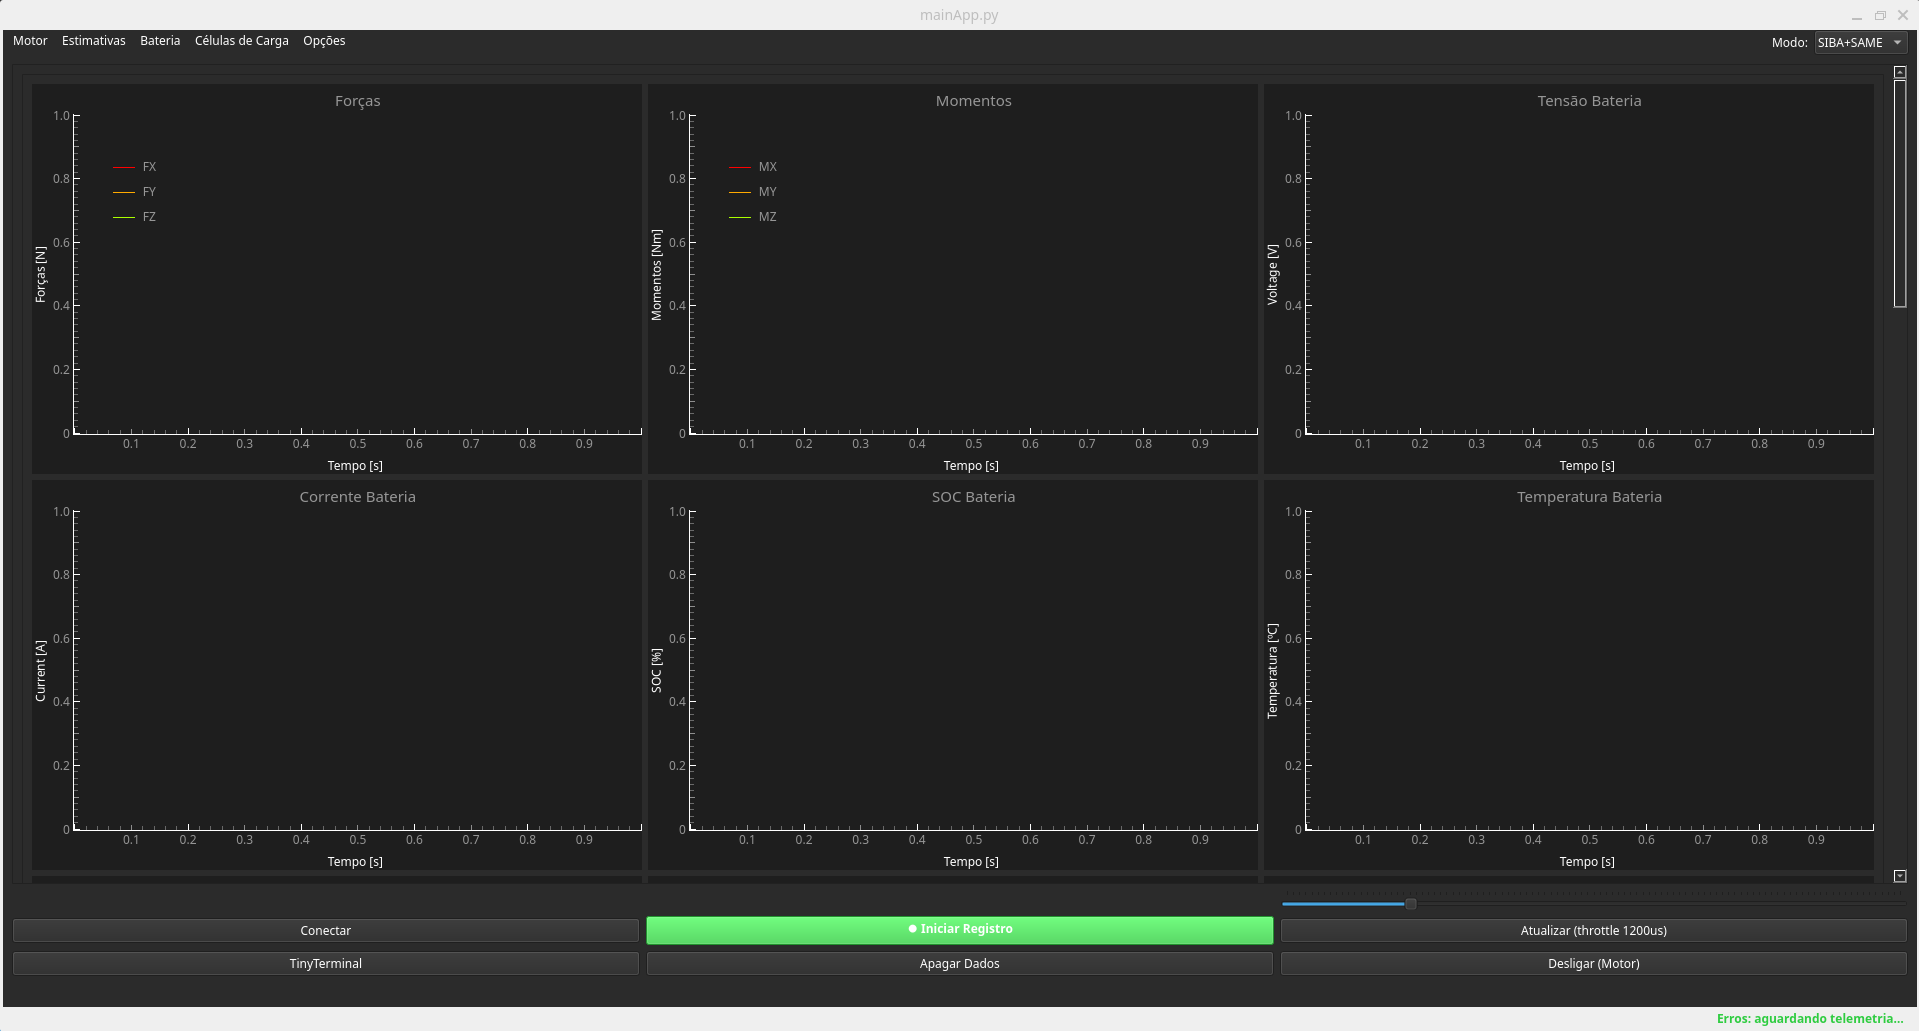
\includegraphics[width=0.85\textwidth]{Textuais/Imgs/Metodologia/gui tela principal.png}
    \fonte{Autor (2026)}
\end{figure}

\begin{figure}[H]
    \centering
    \caption{Interface de supervisão: \textit{TinyTerminal}}
    \label{fig:gui_tinyterminal}
    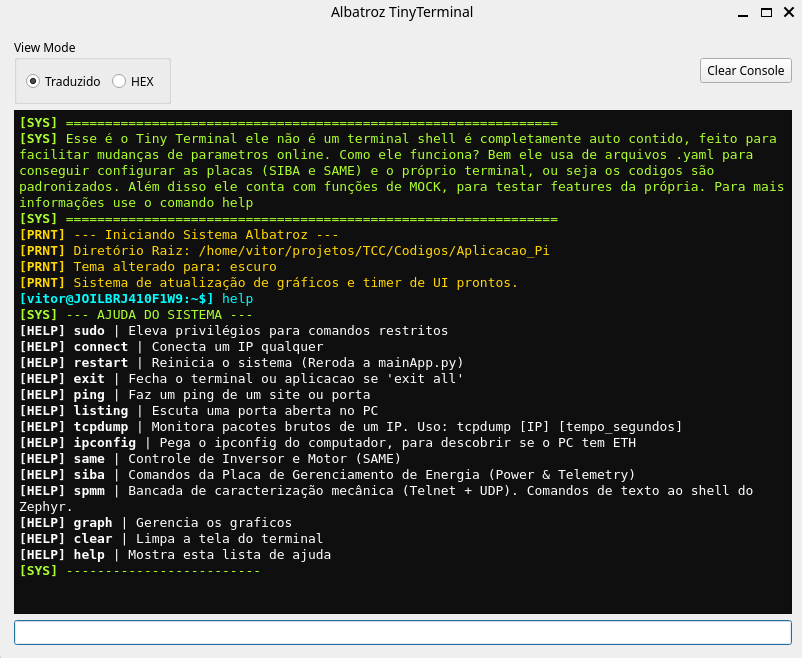
\includegraphics[width=0.85\textwidth]{Textuais/Imgs/Metodologia/gui tiny terminal.png}
    \fonte{Autor (2026)}
\end{figure}

\begin{figure}[H]
    \centering
    \caption{Interface de supervisão: gerenciador de placas}
    \label{fig:gui_gerenciador_placas}
    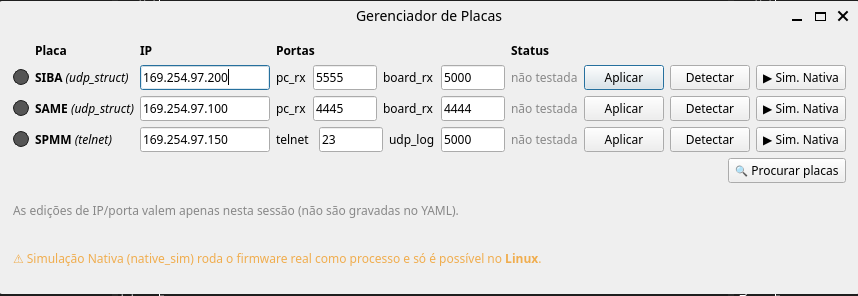
\includegraphics[width=0.85\textwidth]{Textuais/Imgs/Metodologia/gui gerenciador de placas.png}
    \fonte{Autor (2026)}
\end{figure}

\begin{figure}[H]
    \centering
    \caption{Interface de supervisão: painel de erros e alarmes}
    \label{fig:gui_erros_alarmes}
    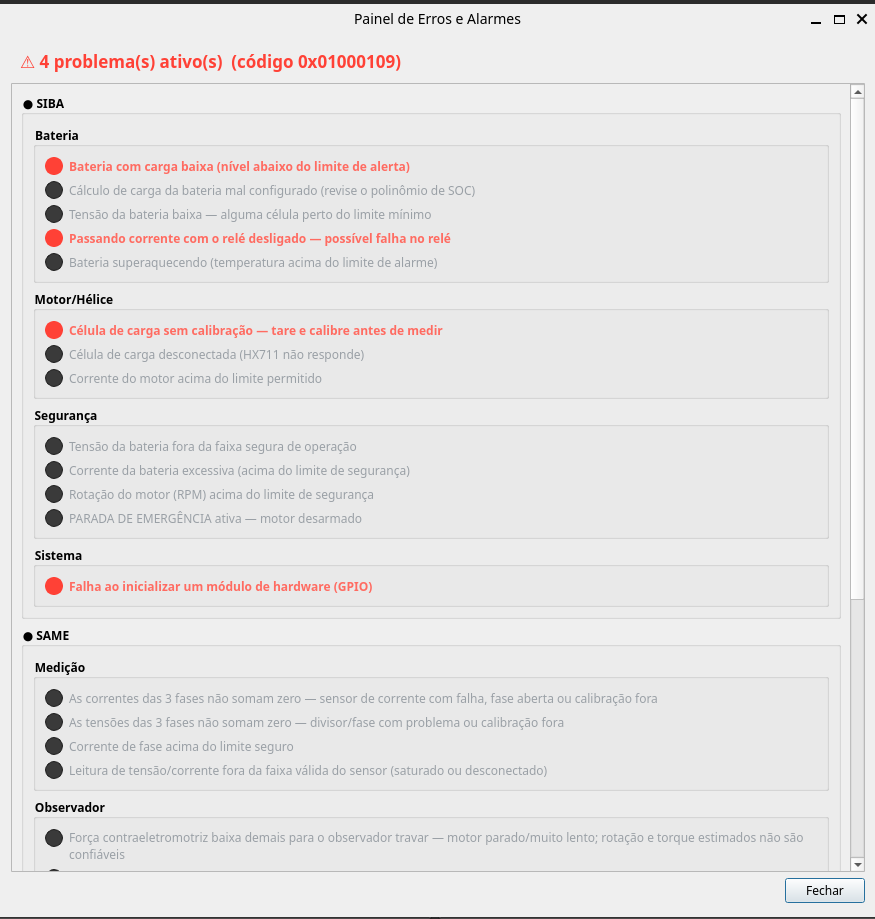
\includegraphics[width=0.85\textwidth]{Textuais/Imgs/Metodologia/gui painel erro e alarmes.png}
    \fonte{Autor (2026)}
\end{figure}

\begin{figure}[H]
    \centering
    \caption{Interface de supervisão: configuração de ganho e \textit{offset} dos sensores}
    \label{fig:gui_sensores}
    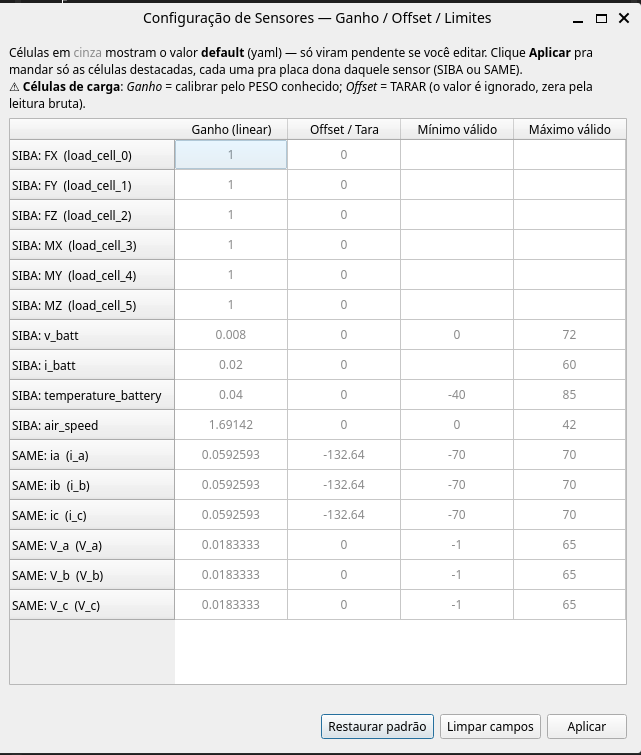
\includegraphics[width=0.85\textwidth]{Textuais/Imgs/Metodologia/gui ganho e offset.png}
    \fonte{Autor (2026)}
\end{figure}

\begin{figure}[H]
    \centering
    \caption{Interface de supervisão: calibração de célula de carga}
    \label{fig:gui_calibrar_celula}
    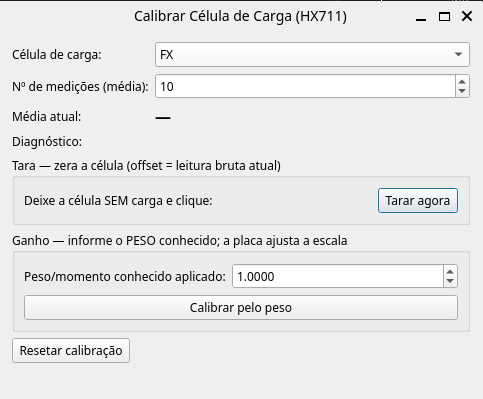
\includegraphics[width=0.85\textwidth]{Textuais/Imgs/Metodologia/gui calibrar celula de carga.png}
    \fonte{Autor (2026)}
\end{figure}

\begin{figure}[H]
    \centering
    \caption{Interface de supervisão: estimação dos ganhos do SMO}
    \label{fig:gui_ganho_smo}
    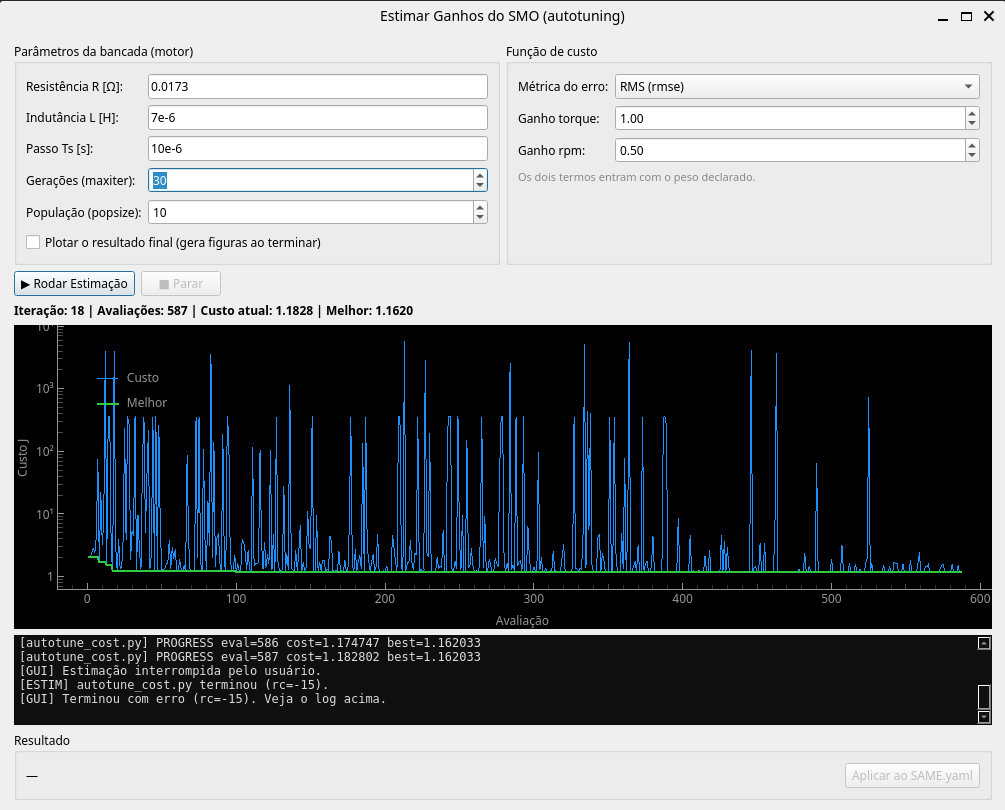
\includegraphics[width=0.85\textwidth]{Textuais/Imgs/Metodologia/gui ganho_smo.png}
    \fonte{Autor (2026)}
\end{figure}

\begin{figure}[H]
    \centering
    \caption{Interface de supervisão: cálculo do coeficiente de tração da hélice}
    \label{fig:gui_helice}
    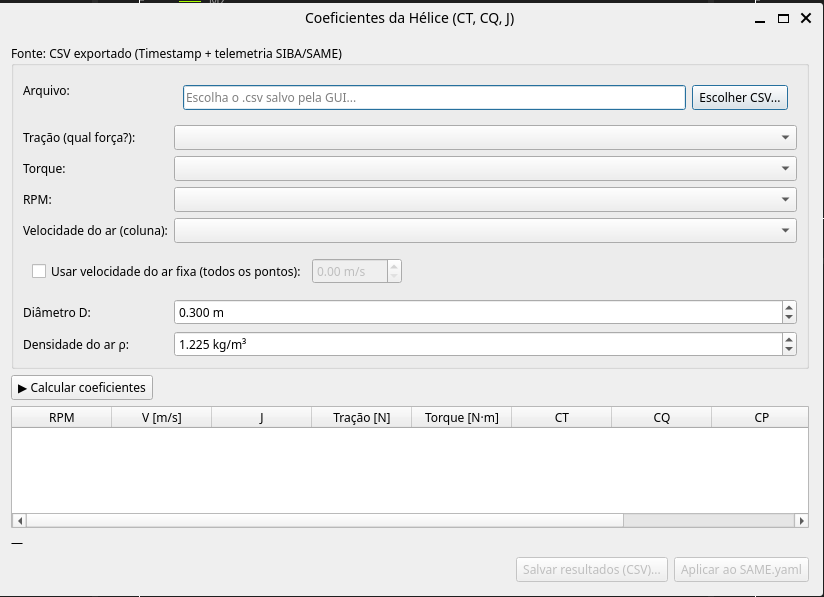
\includegraphics[width=0.85\textwidth]{Textuais/Imgs/Metodologia/gui calculo coeficiente helice.png}
    \fonte{Autor (2026)}
\end{figure}

\begin{figure}[H]
    \centering
    \caption{Interface de supervisão: criação de perfil de motor}
    \label{fig:gui_criar_motor}
    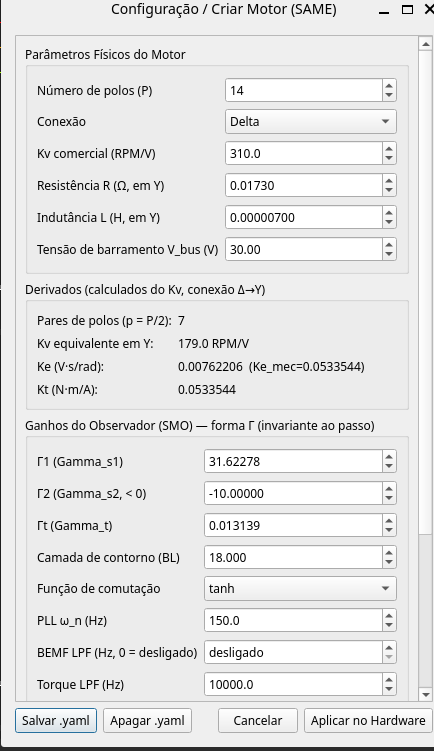
\includegraphics[width=0.85\textwidth]{Textuais/Imgs/Metodologia/gui criar motor.png}
    \fonte{Autor (2026)}
\end{figure}

Para que essa parametrização interativa e o monitoramento operem com alta confiabilidade, mitigando erros de interpretação de dados entre diferentes plataformas, o sistema adota uma estratégia de padronização baseada na linguagem de serialização YAML (\textit{YAML Ain't Markup Language}). A implementação utiliza arquivos de descrição que definem as estruturas fundamentais de telemetria (\textit{logs}), comandos (\textit{CMD}) e configurações da interface.

A configuração do projeto fica em arquivos YAML, e a
\autoref{fig:yaml_example_config} mostra quem usa cada um. O arquivo de
protocolo da placa de medição descreve comandos, telemetria, sensores e
limites, e é usado em dois momentos: na compilação, o \textit{script} \textit{generate.py}
gera a partir deles os cabeçalhos C do \textit{firmware}; na execução, o
\textit{TinyTerminal} os lê para converter um comando de texto no mesmo
pacote binário. Como o \textit{firmware} e a interface partem do mesmo arquivo,
os dois lados interpretam os pacotes da mesma forma. Os demais arquivos são só
da interface: \textit{commands.yaml} define os comandos do
\textit{TinyTerminal}, \textit{plots.yaml} associa as variáveis de telemetria
aos gráficos e \textit{user\_prefs.yaml} guarda as preferências da janela
principal. Os diálogos de calibração e estimação gravam os parâmetros
obtidos (motor, hélice e ganhos do observador) em perfis YAML, que assim ficam
disponíveis na sessão seguinte.

O pacote de telemetria (\texttt{TELEMETRY\_LOG}) enviado em sentido inverso
segue a mesma lógica de geração, com campos específicos por placa.

\begin{figure}[H]
    \centering
    \caption{Fluxo de uso dos arquivos YAML para configuração integrada da GUI e do \textit{firmware}.}
    \label{fig:yaml_example_config}
    \resizebox{0.92\textwidth}{!}{%
    \begin{tikzpicture}[font=\small, >=Latex,
        arq/.style={draw, fill=yellow!15, rounded corners=2pt, minimum width=3.0cm, minimum height=0.75cm, font=\small\itshape},
        uso/.style={draw, thick, rounded corners, align=center, minimum width=4.4cm, minimum height=1.2cm, fill=white},
        le/.style={->, thick},
        lg/.style={<->, thick, densely dashed}]
        % arquivos (centro)
        \node[arq] (same) at (0,4)   {perfis (motor, hélice)};
        \node[arq] (siba) at (0,2.9) {protocolo da placa};
        \node[arq] (cmds) at (0,1.8) {commands.yaml};
        \node[arq] (plot) at (0,0.7) {plots.yaml};
        \node[arq] (pref) at (0,-0.4){user\_prefs.yaml};
        % compilação (esquerda)
        \node[uso] (gen) at (-5.2,3.45) {\textit{generate.py}\\{\footnotesize gera os cabeçalhos C}};
        \node[uso, fill=black!5] (fw) at (-5.2,1.2) {\textit{Firmware} da placa\\de medição};
        \draw[le] (siba.west) -- (gen.east |- siba.west);
        \draw[le] (gen) -- (fw);
        % execução (direita)
        \node[uso] (dial) at (5.6,4.6) {Diálogos de calibração\\e estimação};
        \node[uso] (tiny) at (5.6,2.5) {\textit{TinyTerminal}\\{\footnotesize texto $\to$ CMD binário}};
        \node[uso] (main) at (5.6,0.3) {Janela principal\\{\footnotesize gráficos e preferências}};
        \draw[lg] (same.east) -- (dial.west);
        \draw[le] (siba.east) -- (tiny.west);
        \draw[le] (cmds.east) -- ([yshift=-3mm]tiny.west);
        \draw[le] (plot.east) -- ([yshift=2mm]main.west);
        \draw[lg] (pref.east) -- ([yshift=-2mm]main.west);
        % grupos
        \begin{scope}[on background layer]
            \node[draw=gray, dashed, rounded corners, fill=blue!3, fit=(gen)(fw), inner sep=8pt,
                  label={[font=\small\bfseries]above:Compilação}] {};
            \node[draw=gray, dashed, rounded corners, fill=green!4, fit=(dial)(tiny)(main), inner sep=8pt,
                  label={[font=\small\bfseries]above:Execução (interface)}] {};
        \end{scope}
        % legenda
        \draw[le] (-2.2,-1.6) -- ++(0.8,0) node[right, font=\footnotesize] {lê};
        \draw[lg] (0.2,-1.6) -- ++(0.8,0) node[right, font=\footnotesize] {lê e grava};
    \end{tikzpicture}%
    }

    Fonte: Autor (2026).
\end{figure}

A calibração de um sensor usa o mesmo caminho de tradução do
\textit{TinyTerminal} (\autoref{fig:tinyterminal_fluxo}): o operador edita
um valor (ganho, deslocamento de zero ou limite de segurança) na tela de
configuração de sensores, e esse valor é traduzido no mesmo formato de
comando usado em todo o resto do sistema, enviado pela rede até a placa
de medição, que aplica o ajuste ao canal do sensor indicado. A
\autoref{fig:seq_calibracao} resume essa sequência completa, da edição na
tela até a confirmação. Não existe uma mensagem de confirmação separada: a
mudança só é percebida no próximo pacote de telemetria, quando a leitura
daquele canal passa a refletir o novo valor (por exemplo, uma célula de
carga recém-tarada passa a ler próximo de zero). A placa grava esses
ajustes, junto com os parâmetros do observador, numa memória não volátil
(EEPROM): ao ser religada, restaura os valores salvos em vez de voltar ao
padrão do arquivo de configuração (\autoref{fig:yaml_example_config}).

\begin{figure}[H]
    \centering
    \caption{Sequência de calibração de um sensor, da interface à confirmação por telemetria}
    \label{fig:seq_calibracao}
    \resizebox{\textwidth}{!}{%
    \begin{tikzpicture}[
        font=\scriptsize,
        actor/.style={draw, rounded corners, align=center, minimum width=2.3cm, minimum height=0.7cm},
        lifeline/.style={dashed, gray},
        msg/.style={-{Latex}, thick}
    ]
        \node[actor] (dlg) at (0,0)   {Tela de\\configuração};
        \node[actor] (term) at (2.8,0) {Tradução para\\comando padrão};
        \node[actor] (nci) at (5.6,0) {Rede\\(placa recebe)};
        \node[actor] (core) at (8.4,0) {Firmware aplica\\no sensor};
        \node[actor] (tel) at (11.2,0) {Telemetria};
        \node[actor] (gui) at (14.0,0) {Interface\\(operador)};

        \foreach \n in {dlg,term,nci,core,tel,gui}
            \draw[lifeline] (\n.south) -- ++(0,-4.6);

        \draw[msg] (0,-1.0)  -- (2.8,-1.0) node[midway, above, font=\tiny]{placa, sensor, campo, valor};
        \draw[msg] (2.8,-1.9) -- (5.6,-1.9) node[midway, above, font=\tiny]{comando binário};
        \draw[msg] (5.6,-2.8) -- (8.4,-2.8) node[midway, above, font=\tiny]{identifica o sensor e o ajuste};
        \draw[msg] (8.4,-3.7) -- (11.2,-3.7) node[midway, above, font=\tiny]{canal atualizado};
        \draw[msg] (11.2,-4.4) -- (14.0,-4.4) node[midway, above, font=\tiny]{leitura refletindo o novo ganho};
    \end{tikzpicture}%
    }

    Fonte: Autor (2026)
\end{figure}

